\documentclass[a4paper,12pt]{article}

\usepackage[utf8x]{inputenc}
\usepackage[italian]{babel}
\usepackage{graphicx}

%opening
\title{Fisica dei Sistemi Complessi\\Relazione di progetto\\3D Network Visualizator}
\author{Giacomo Benvenuti\\Enrico D'Angelo\\Fabrizio Nuzzo}
\date{}

\begin{document}

\maketitle

\begin{abstract}
La visualizzazione dei dati \`e lo studio della rappresentazione visuale dei dati stessi, lo scopo principale \`e quello di comunicare le informazioni contenute nei dati in maniera chiara ed efficace. Per trasmettere le informazioni sia l'estetica che la funzionalità della visualizzazione devono andare di pari passo, in modo da fornire la comprensione delle informazioni contenute in un dataset altrimenti complesso da comprendere. Lo scopo fondamentale della visualizzazione dei dati \`e quindi la comunicazione degli aspetti chiave del dataset in una maniera più intuitiva.

Il progetto svolto ha lo scopo di visualizzare le interazioni che avvengono nei diversi istanti tra i nodi di una rete. 3D-Network-Visualizator visualizza queste interazioni in maniera grafica. I nodi che compongono la rete sono disposti in uno spazio tridimensionale secondo le loro coordinate. Le interazioni vengono visualizzate come degli archi che vanno da un nodo all'altro dando una diversa ampiezza all'arco in base alla frequenza dell'interazione, per meglio capire a colpo d'occhio l'importanza relativa delle diverse interazioni. Infine gli istanti scorrono su una linea temporale dando la possibilità di visualizzare come in un video i cambiamenti che avvengono nelle interazioni tra i diversi nodi.
\end{abstract}

\section{Il Problema}
L'uomo per sua natura ha una spiccata capacit\`a d'analisi critica ma questa deve essere supportata da una chiara ed appropriata visualizzazione dei dati.

Osservando direttamente un dataset che rappresenta una rete e le interazioni che avvengono tra i suoi nodi, anche se di dimensioni modeste, non \`e immediato rispondere a domande quali: “quali sono le interazioni che avvengono?”, “quali nodi sono quelli con maggiori o minori interazioni?”, “esistono delle interazioni ricorrenti tra certi nodi?” Che sono solo alcune delle domande di interesse per chiunque si trovi ad analizzare un dataset di questo tipo.

% \subsection{Una possibile soluzione}
% Un modo semplice per rappresentare una rete consiste nell'utilizzare una tabella con l'elenco di tutti i nodi della rete riportato sia nelle righe che nelle colonne. In questo modo nella cella che incrocia due nodi viene riportato il valore che rappresenta l'interazione avvenuta tra quei due nodi. Una tabella pu\`o per\`o rappresentare lo stato delle interazioni della rete in un solo istante, per poter osservare le interazioni nel tempo occorre quindi utilizzare una tabella per ogni istante.
% 
% \subsection{Considerazioni}
% Nonostante questo approccio sia molto semplice, non e' auspicabile perché inefficiente dal punto di vista computazionale e della leggibilità dei risultati; Se per esempio volessimo rappresentare le interazioni che avvengono in ogni istante di tempo che non coinvolgono tutte le coppie di nodi, le tabelle risulterebbero sparse, perci\`o viene utilizzata una gran quantità di memoria per memorizzare in realtà una piccola quantità di informazione. Questo problema viene ulteriormente peggiorato quando la rete contiene un gran numero di nodi.

\section{3D-Network-Visualizator}
3D-Network Visualizator visualizza le interazioni tra i nodi di una rete in modo pratico e intuitivo. I nodi venogno disposti in uno spazio tridimensionale in base alle loro coordinate. La visualizzazione dei diversi istanti di tempo avviene in maniera fluida come se si stesse guardando un video. Le interazioni tra i nodi sono rappresentate con degli archi che collegano coppie di nodi. Le interazioni sono evidenziate con colori differenti, con archi di altezza differente in base alla frequenza dell'interazione che rappresentano. Ogni arco evidenzia anche la direzione dell'interazione e la quantit\`a delle interazioi che avvengono in un dato istante.

3D-Network Visualizator permette quindi di comprendere a colpo d'occhio le caratteristiche delle interazioni. \`E facile vedere, ad esempio, quali siano le interazioni con maggiore frequenza, o se alcuni nodi hanno interazioni sporadiche o meno.

Il software permette anche di concentrare la visualizzazione su un sottoinsieme dei nodi, evidenziando maggiormente le interazioni che coinvolgono questi nodi e mettendo in secondo piano tutte le altre. La visualizzazione avviene in uno spazio tridimensionale ed \`e quindi possibile spostare l'angolo di visualizzazione della rete in tutte le dimensioni se questo pu\`o aiutare la visualizzazione della rete.

\subsection{Specifiche di funzionamento}
Le specifiche di funzionamento di 3D-Network Visualizator sono:
\begin{itemize}
 \item i nodi che compongono la rete vengono posizionati in base alle loro coordinate.
 \item i nodi possono essere disposti in uno spazio piano o in uno spazio sferico.
 \item le interazioni tra i nodi vengono visualizzate come archi, l'altezza degli archi \`e direttamente proporzionale alla frequenza delle interazioni.
 \item deve essere evidenziata la direzione delle interazioni.
 \item deve essere evidenziata la quantit\`a delle interazioni.
\end{itemize}

Per una buona visualizzazione, ed analisi, della rete sono state implementate anche le seguenti specifiche:
\begin{itemize}
 \item \`e possibile selezionare un sottoinsieme dei nodi durante la visualizzazione per concentrarsi sulle loro interazioni.
 \item l'angolo di visualizzazione nello spazio tridimensionale pu\`o essere spostato in tutte le dimensioni.
 \item \`e possibile variare il tempo impiegato per la visualizzazione di un istante di tempo (ha l'effetto di velocizzare o rallentare l'animazione).
\end{itemize}

\section{Tecnologie utilizzate}
Per la realizzazione di questo progetto sono state utilizzate diverse tecnologie:
\begin{description}
 \item[Processing:] \`e una libreria Java di sviluppo sotto licenza GNU LGPL. La libreria viene incontro a necessità di utilizzo più specifico dal punto di vista grafico. Le molteplici possibilità della libreria combaciano perfettamente con le nostre aspettative di rappresentazione grafica del progetto. Processing viene oggi utilizzato da studenti, artisti, designers, ricercatori e obbisti per produrre prototipi e prodotti finiti di livello professionale. Processing \`e stato inizialmente sviluppato da Ben Fry e Casey Reas nel 2001 mentre erano entrambi studenti sotto la supervisione di John Maeda al MIT Media Lab. Ulteriore sviluppo di Processing ha avuto luogo all'Interaction Design Institute Ivrea, Carnegie Mellon University, e alla UCLA, dove Reas \`e capo del Dipartimento di Design | Media Arts. Miami University, Oblong Industries, e la fondazione Rockefeller hanno contribuito finanziando il progetto.
 \item[XML:] (eXtensible Markup Language). XML \`e un linguaggio di markup molto pratico per l'elaborazione da parte di un calcolatore, facilemnte leggibile da parte dell'uomo, e indipendente dal linguaggio di programmazione usato per elaborarlo. Per questi motivi \`e stato scelto
 \item[Java] linguaggio di programmazione orientato agli oggetti, indipendente dalla piattaforma. Grazie all'uso di Java lo stesso codice pu\`o essere eseguito su macchine Windows, Linux, MacOSX.
\end{description}
        
\section{Implementazione}

\subsection{Il dataset}
Il tipo di dataset che viene visualizzato contiene tutte le informazioni che riguardano i nodi che compongono la rete, e istante per istante, tutte le interazioni che avvengono tra i nodi.
Gli attributi che riguardano i nodi sono:
\begin{description}
 \item[l'identificativo] \`E un identificativo numerico che viene utilizzato all'interno del dataset per indicare uno specifico nodo. Ogni nodo possiede un identificativo univoco.
 \item[l'etichetta] L'etichetta svolge circa lo stesso ruolo dell'identificativo ma \`e più adatta per essere memorizzata dalle persone. gli identificativi servono al software per distinguere e identificare i diversi nodi, per questo motivo sono degli indici numerici. Per una persona \`e invece molto più facile memorizzare degli identificativi alfanumerici, e questo \`e lo scopo delle etichette. Inoltre quando i nodi rappresentano delle entita fisiche esistenti, come ad esempio delle città, \`e utile che le label rispecchino il nome di tale entità al fine di aiutare la comprensione del fenomeno. L'etichetta di un nodo non deve necessariamente essere univoca.
 \item[coordinate] Sono le coordinate cartesiane dei nodi.
\end{description}

Gli attributi che riguardano le interazioni sono:
\begin{description}
 \item[la sorgente] \`E l'identificativo del nodo da cui ha origine l'interazione.
 \item[l'obiettivo] \`E l'identificativo del nodo obiettivo dell'interazione.
 \item[quantità] Rappresenta la quantità del flusso che costituisce l'interazione. Cosa sia effettivamente il flusso che costituisce l'interazione dipende dal tipo di rete in esame. Pu\`o per esempio trattarsi di pacchetti scambiati da diversi elaboratori collegati via rete, o di automobili che si spostano da un luogo ad un altro.
 \item[frequenza] \`E la frequenza che caratterizza l'interazione.
\end{description}

Le informazioni che riguardano le interazioni sono naturalmente suddivise per istanti. Anche gli istanti hanno degli attributi:
\begin{description}
 \item[valore] \`E l'identificativo dell'istante. Gli identificativi degli istanti devono essere univoci e consecutivi.
 \item[etichetta] Anche in questo caso le etichette servono per meglio comprendere il fenomeno. Le etichette possono infatti rispecchiare il tempo fisico, l'ora, in cui sono state prese le misurazioni che costituiscono le informazioni riguardanti le interazioni.
\end{description}
 
\subsection{Il file network XML}
 
L'input del nostro visualizzatore \`e un file che contiene la descrizione della topologia di una rete e le interazione che avvengono tra i suoi nodi. Come formato del file di input abbiamo scelto l'XML per diversi motivi. In primo luogo per la facilità con cui pu\`o essere processato da un calcolatore. In secondo luogo per la sua portabilità su diverse piattaforme e linguaggi di programmazione, in questo modo lo stesso file di input pu\`o essere utilizzato facilmente anche da altri software scritti in altri linguaggi di programmazione per altre piattaforme software. Infine per la sua caratteristica di essere facilmente leggibile anche dall'uomo.
Il pricipale punto a sfavore di questo formato \`e la scarsa compattezza, nel senso che oltre alle informazioni relative alla rete il file contiene anche molte meta-informazioni che servono appunto per facilitare l'elaborazione del file e facilitarne la sua leggibilità. Questo significa che per file di input che rappresentano reti di grandi dimensioni, ad esempio con migliaia di nodi e centinaia di interazioni, molto spazio per la memorizzazione del file su disco sarà occupato dalle meta-informazioni. In questi casi un formato binario sarebbe stato sicuramente più compatto, ma avrebbe perso tutte le caratteristiche positive elencate sopra.
 
Qui di seguito viene riportato un file di input di esempio:
\begin{verbatim}
<?xml version="1.0" encoding="UTF-8"?>
<network>
 <static-data>
   <network-name>new-test-02</network-name>
   <nodes-list>
     <node id="0" label="192.168.0.1" x="2" y="0" z="6" />
     <node id="1" label="192.168.0.2" x="3" y="0" z="8" />
   </nodes-list>
   <flat>true</flat>
 </static-data>
 <dynamic-data>
   <instant value="0" label="0">
     <interaction source="1" target="0" quantity="1" frequency="0.6080425" />
   </instant>
   <instant value="1" label="1">
     <interaction source="1" target="0" quantity="8" frequency="1.31866568" />
   </instant>
 </dynamic-data>
</network>
\end{verbatim}

La struttura del file di input \`e divisa in due parti principali:
\begin{description}
 \item[static-data:] Questa parte contiene le informazioni statiche della rete, cio\`e la sua topologia, \`e composta dai seguenti elementi:
 \begin{itemize}
  \item network-name: il nome della rete
  \item nodes-list: l'elenco dei nodi presenti nella rete
  \item flat: indica se la rete deve essere visualizzata in uno spazio piano o sferico
 \end{itemize}
Ogni nodo in nodes-list \`e descritto con i seguenti attributi:
 \begin{itemize}
  \item id: \`e l'identificativo univoco del nodo
  \item label: \`e l'etichetta del nodo
  \item x, y e z: sono le coordinate del nodo.
 \end{itemize}
 \item[dynamic-data:] Questa parte contiene tutte le informazioni dinamiche della rete, cio\`e le interazioni che avvengono tra i suoi nodi. \`E strutturata come una lista di istanti. Ogni istante \`e strutturato come una lista di interazioni. Ogni interazione \`e descritta con i seguenti attributi:
 \begin{itemize}
  \item source: \`e l'identificativo del nodo dal quale parte l'interazione
  \item target: \`e l'identificativo del nodo obiettivo dell'interazione
  \item quantity: rappresenta la quantità di dati scambiati durante l'interazione
  \item frequency: \`e la frequenza dell'interazione
 \end{itemize}
\end{description}
 
\subsection{Creazione di una nuova rete}
3D-Network-Visualizator permettere di creare una nuova rete che potr\`a poi essere visualizzata. In \figurename~\ref{fig:createnetwork} viene riportata l'interfaccia della creazione di una nuova rete alla quale \`e possibile accedere tramite il menu  \textit{File} $\rightarrow$ \textit{crea una nuova rete}.

\begin{figure}[htb!]
 \begin{center}
  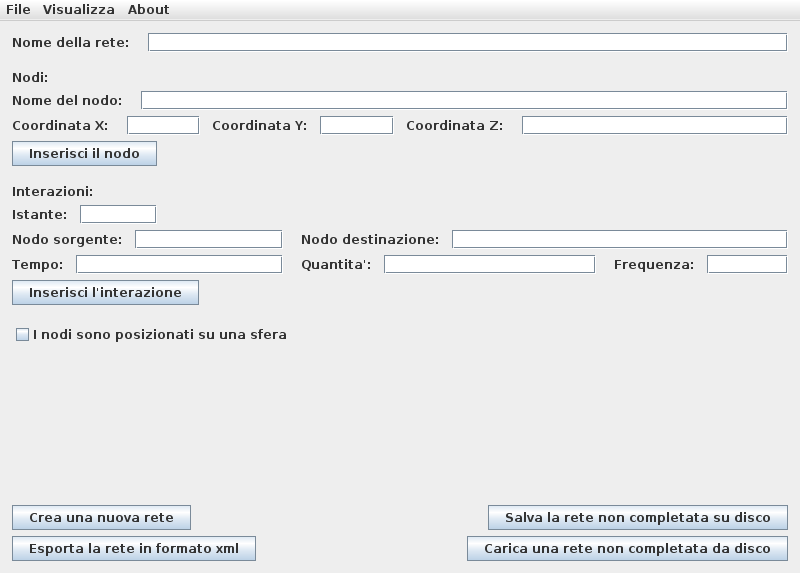
\includegraphics[width=\textwidth]{images/create-network.png}
 \end{center}
 \caption{Form per la creazione di una nuova rete.}
 \label{fig:createnetwork}
\end{figure}

\begin{itemize}
 \item Il campo ``Nome della rete'' indica sia il nome della rete che il nome del file che sar\`a prodotto.
 \item Il campo ``Nome del nodo'' indica l'etichetta del nodo che stiamo inserendo.
 \item I campi ``coordinata X, Y e Z'' indicano ovviamente il valore delle coordinate X, Y e Z.
\end{itemize}
Una volta inseriti i valori relativi ad uno nodo, cliccando sul pulsante \textit{Inserisci il nodo}, le informazioni relative al nodo verranno memorizzate, i campi torneranno vuoti e sar\`a possibili inserire i dati relativi ad un altro nodo.

\begin{itemize}
 \item Il campo ``Istante'' indica l'identificativo dell'istante a cui si intende aggiungere un'interazione.
 \item Il campo ``Nodo sorgente'' indica l'etichetta del nodo dal quale ha inizio l'interazione.
 \item Il campo ``Nodo destinazione'' indica l'etichetta del nodo obiettivo dell'interazione.
 \item Il campo ``Tempo'' indica l'etichetta dell'istante. Pu\`o rappresentare, ad esempio, il tempo reale in cui sono state prese le misurazione.
 \item Il campo ``Quantit\`a'' indica la quantit\`a delle interazioni.
 \item Il campo ``Frequenza'' indica la frequenza delle interazioni.
\end{itemize}
Anche in questo caso cliccando sul pulsante \textit{Inserisci l'interazione} tutte le informazioni inserite vengono memorizzate e i campi vengono liberati per poter inserire una nuova interazione.

Il checkbox con etichetta ``I nodi sono posizionati su una sfera'' indica ovviamente, come dice l'etichetta, se i nodo sono o meno posizionati su una sfera.

Il pulsante \textit{Salva la rete non completata su disco} permette di memorizzare in un file i progressi finora fatti nella creazione di una rete. Non viene generato un file di input per il visualizzatore, questa funzionalit\`a \`e pensata per permettere all'utente di creare una rete di input in pi\`u tempi.

Il pulsante \textit{Carica una rete non completata da disco} permette invece di caricare una rete incompleta, memorizzata precedentemente, e di continuare con l'inserimento dei nodi e delle interazioni.

Una volta che tutti i dati sono stati inseriti si pu\`o cliccare sul pulsante \textit{Esporta le rete in formato xml} per creare un file di input per il visualizzatore. A questo punto \`e possibile visualizzare la rete appena creata.

Il pulsante \textit{Crea una nuova rete} invece serve per annullare tutte le modifiche fatte finora e ricominciare daccapo con la creazione di una nuova rete.

\subsection{Importare una rete}
Tramite il menu \textit{File} $\rightarrow$ \textit{Importa una nuova rete} \`e possibile caricare una file di input che rappresenta una rete e le interazioni tra i suoi nodi.

\begin{figure}[htb!]
 \begin{center}
  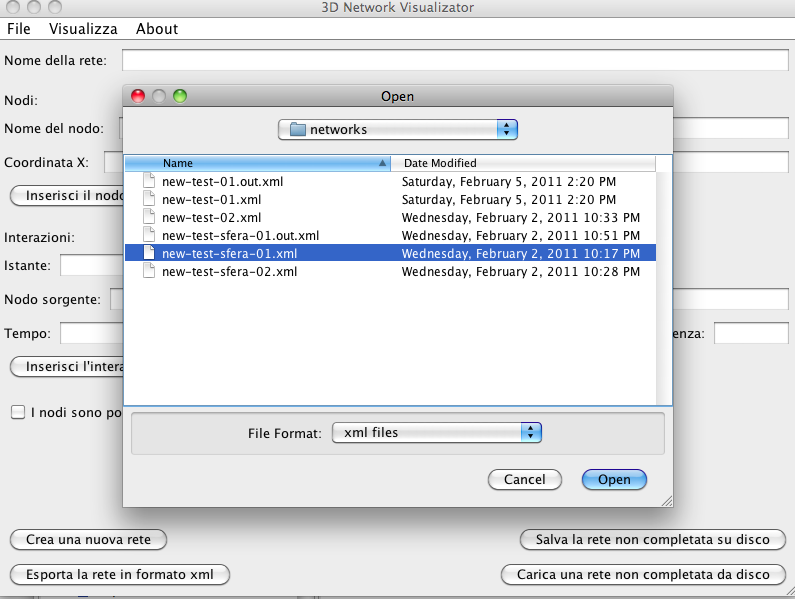
\includegraphics[width=\textwidth]{images/image0.png}
 \end{center}
 \caption{File dialog per importare una nuova rete.}
 \label{fig:importnetwork}
\end{figure}

Una volta importato il file, il programma inizier\`a a visualizzare la rete con una breve animazione introduttiva, finita l'animazione sar\`a possibile far partire la simulazione tramite il tasto \textit{play} posizionato nella barra dei comandi (\figurename~\ref{fig:slider}). 

In qualsiasi momento \`e possibile mettere in pausa la simulazione tramite il tasto \textit{pause}, in questo modo sar\`a possibile soffermarsi sulla visualizzazione dell'istante corrente ed analizzare con cura tutte le interazioni.

Uno slider posto di fianco alla barra dei comandi (\figurename~\ref{fig:slider}) mostra l'avanzamento della simulazione. 

Tramite il campo situato a fianco lo slider \`e possibile cambiare la durata di visualizzazione di un istante, questa opzione permette di velocizzare o rallentare l'animazione.
 
\begin{figure}[htb!]
 \begin{center}
  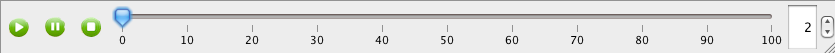
\includegraphics[width=\textwidth]{images/image1.png}
 \end{center}
 \caption{Slider per controllare l'animazione delle interazioni.}
 \label{fig:slider}
\end{figure}
 
\subsection{Opzioni di Visualizzazione}
Tramite il menu \textit{Visualizza} \`e possibile, in ogni momento della visualizzazione, accedere a diverse opzioni di visualizzazioni:
\begin{itemize}
 \item \textit{Visualizza spazio 3D di riferimento (s)} (attiva di default) tramite questa opzione \`e possibile visualizzare/nascondere la griglia di riferimento dello spazio tridimensionale. Questa opzione \`e utile per ridurre al minimo gli elementi presenti nel riquadro che possono interferire con la comprensione del fenomeno visualizzato.
 \item \textit{Mostra solo archi entranti (e)} (disattivata di default) questa opzione permette di visualizzare solo gli archi entranti dei nodi. Quest'opzione risulta utile quando sono selezionati solo alcuni dei nodi che compongono la rete, in questo caso \`e possibile concentrarsi sulle interazioni per cui questi nodi sono l'obiettivo, e non la sorgente.
 \item \textit{Mostra gli archi di tutti i nodi (r)} (attiva di default) questa opzione permette di visualizzare/nascondere tutte le interazioni tra i nodi della rete. Quando sono selezionati dei nodi, quest'opzione ha l'effetto di visualizzare/nascondere tutte le interazioni che si originano dai nodi non selezionati.
 \item \textit{Visualizza tutte le etichette (l)} (disattivata di default) quest'opzione permette di visualizzare/nascondere tutte le etichette di nodi presenti nella rete.
\end{itemize}
\`E possibile attivare/disattivare le stesse opzioni prenendo il tasto corrispondente alla lettere scritta tra parentesi di fianco ai menu.

% Tenendo premuto il tasto \textit{CTRL} e cliccando su un nodo, quest'ultimo viene selezionato. L'effetto di questa operazione \`e che ora tutte le interazioni che si originano in quel nodo sono evidenziate, mentre tutte le altre interazioni passano in secondo piano. \`E possibile selezione diversi nodi contemporaneamente ripetendo quest'operazione. Per deselezionare un nodo occorre cliccare sul nodo stesso tenendo premuto il tasto \textit{Alt}.

Infine, tramite il mouse \`e possibile modificare l'angolo di visualizzazione della rete in tutte le direzioni.

\subsubsection{Visualizzare un sottoinsieme della rete}
% Durante i primi test della nostra applicazione abbiamo notato che era difficoltoso concentrare l'attenzione su una ristretta cerchia di nodi, appunto una  partizione della rete. L'attività della rete cambia ogni istante e la possibilità che le connessioni  interessino tutti  i nodi non \`e remota. Uno scenario del genere \`e sicuramente utile per avere un quadro completo della situazione  in un dato istante ma se la nostra analisi \`e rivolta soltanto a determinati nodi tutte le altre interazioni tra i nodi della rete risultano superflue.
Tenendo premuto il tasto \textit{CTRL} e cliccando su un nodo, quest'ultimo viene selezionato. L'effetto di questa operazione \`e che ora tutte le interazioni che si originano in quel nodo sono evidenziate, mentre tutte le altre interazioni passano in secondo piano. \`E possibile selezione diversi nodi contemporaneamente ripetendo quest'operazione. Per deselezionare un nodo occorre cliccare sul nodo stesso tenendo premuto il tasto \textit{Alt}.

Grazie a questa opzione \`e possibile concentrarsi su una parte della rete e delle sue interazioni senza essere disturbati dalle interazioni che non ci interessano.

La \figurename~\ref{fig:caotica} mostra una rete in cui tutte le interazioni sono visualizzate. Nel caso ci si voglia concentrare solo su alcune di tali interazioni, \`e utili selezionare solo i nodi interessati per ottenere una visualizzazione pi\`u chiara del sistema, come mostrato in figura \figurename~\ref{fig:sottoinsieme}.

\begin{figure}[htb!]
 \begin{center}
  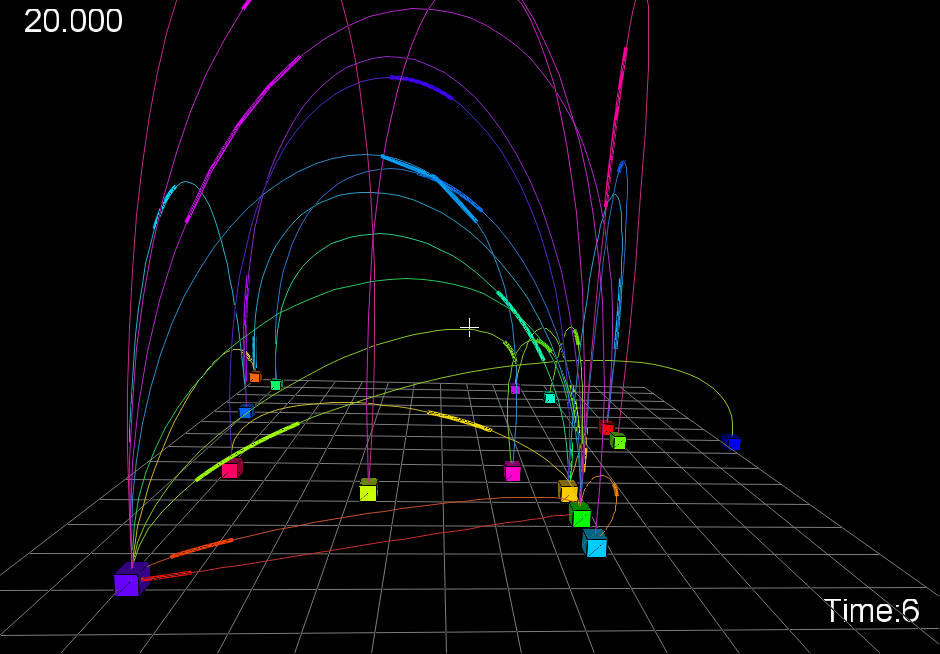
\includegraphics[width=\textwidth]{images/image2.png}
 \end{center}
 \caption{Visualizzazione caotica.}
 \label{fig:caotica}
\end{figure}
 
%Per ovviare a questo problema \`e stata implementata la funzione partizione; 
%Questa funzione \`e disponibile  in qualsiasi momento dell'animazione; per utilizzarla basta portarsi con il cursore sul nodo/i che ci interessano e selezionarli premendo i tasto “ctrl”.

\begin{figure}[htb!]
 \begin{center}
  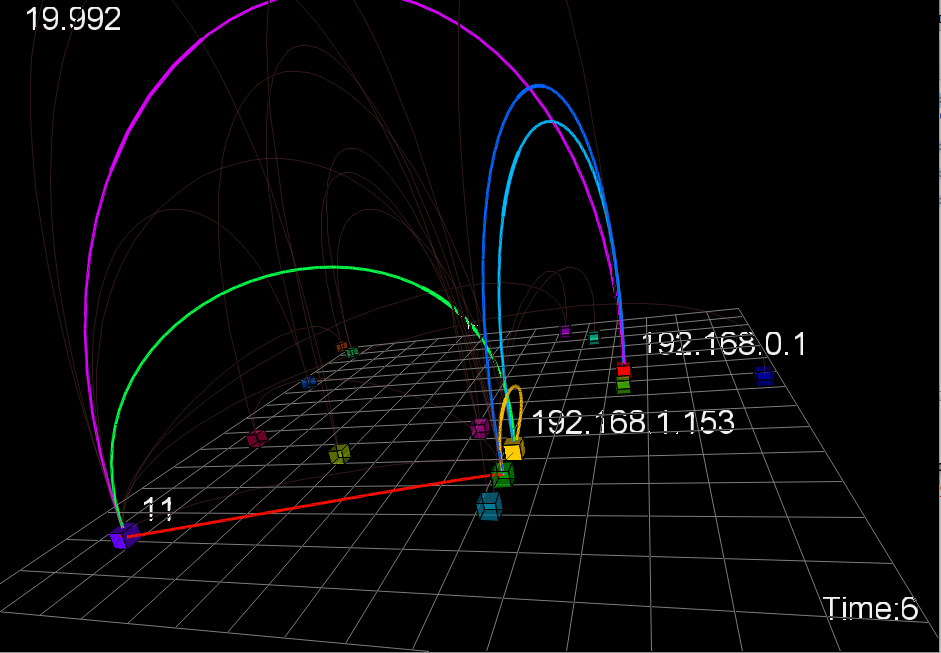
\includegraphics[width=\textwidth]{images/image3.png}
 \end{center}
 \caption{Visualizzazione di un sottoinsieme della rete.}
 \label{fig:sottoinsieme}
\end{figure}
 
%In questo screenshot possiamo notare come la funzione partizione faciliti l'analisi di questa parte del network formata da 3 nodi nell'istante 6 
 
\subsubsection{Visualizzazione dei nodi su un piano e su una sfera}
3D-Network-Visualizator supporta la visualizzazione di nodi che possono essere disposti su un piano o su una sfera. Il secondo caso potrebbe essere utile per visualizzare, ad esempio, i piani di volo intercontinentali.

La \figurename~\ref{fig:piano} mostra un esempio di rete visualizzata su un piano, mentre la \figurename~\ref{fig:sfera} mostra un esempio di rete visualizzata su una sfera.

\begin{figure}[htb!]
 \begin{center}
  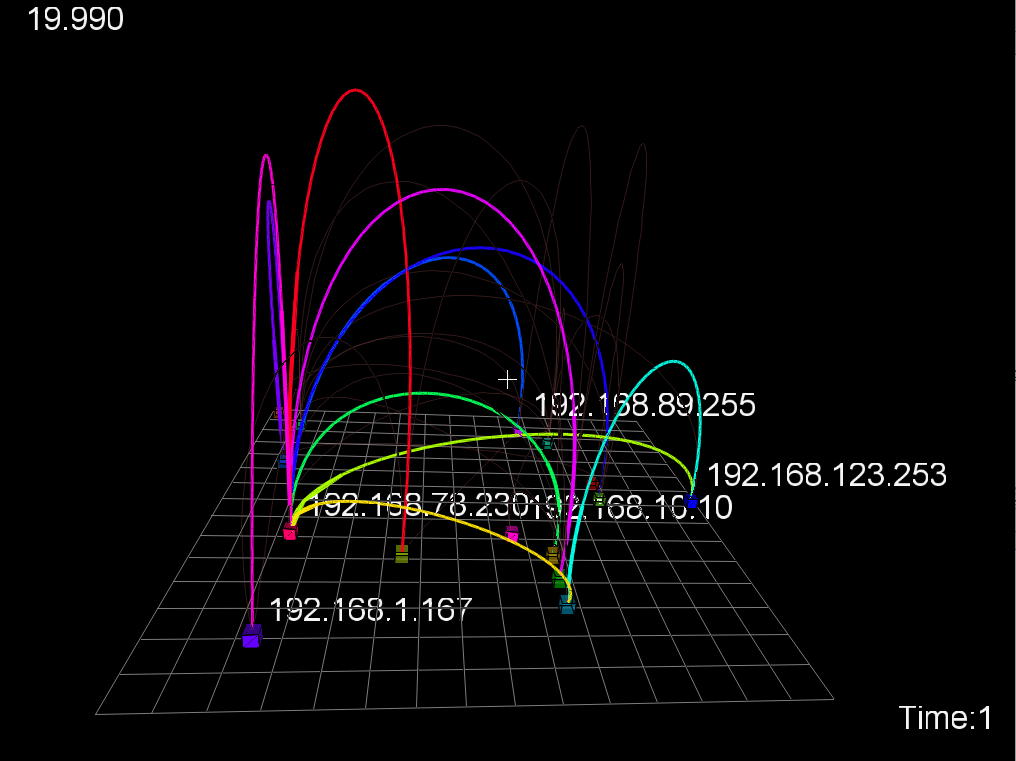
\includegraphics[width=\textwidth]{images/image4.png}
 \end{center}
 \caption{Rete visualizzata su un piano.}
 \label{fig:piano}
\end{figure}

\begin{figure}[htb!]
 \begin{center}
  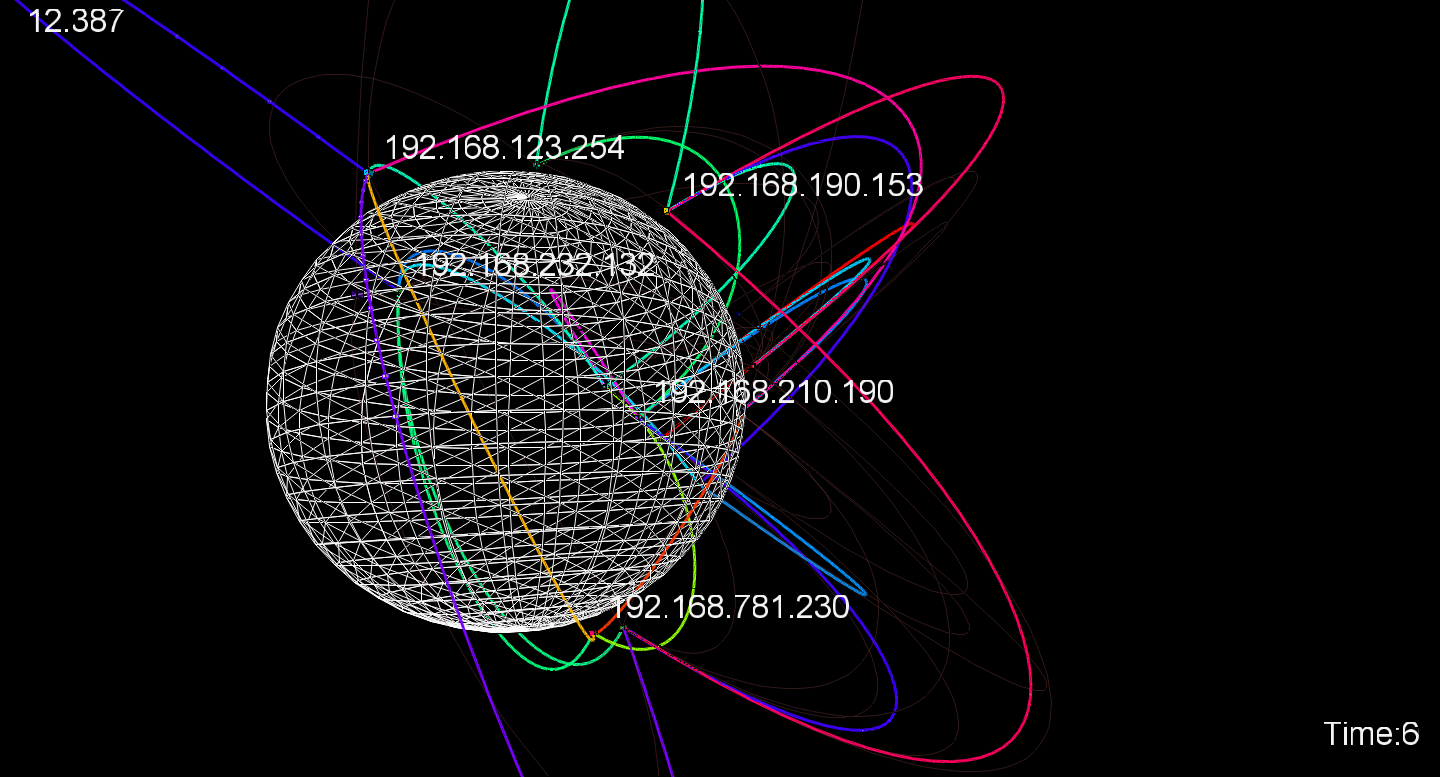
\includegraphics[width=\textwidth]{images/image5.png}
 \end{center}
 \caption{Rete visualizzata su una sfera.}
 \label{fig:sfera}
\end{figure}

\section{Conclusioni}
Lo studio e l'implementazione di 3D-Network-Visualizator ci ha dato la possibilit\`a di scoprire i vantaggi derivanti da un'efficace visualizzazione dei dati. Spesso per analizare un fenomeno non serve avere sotto mano delle statistiche dettagliate e un database contenente l'intero dataset contenente migliaia di entry. Questo per il semplice motivo che viene a mancare una visione d'insieme del fenomeno che potrebbe portare un risultato d'analisi inaspettato.

3D-Network-Visualizator riesce a fornire una visualizzazione chiara delle interazione che avvengono tra i nodi di una rete. Permette di focalizzare l'attenzione solo su un sottoinsieme dei nodi, di guardare alle interazioni che vengono generate da questi nodi o alle interazioni che hanno tali nodi come obiettivo.

L'evoluzione temporale delle interazioni viene presentata come un'animazione che \`e possibile velocizzare, rallentare o fermare per meglio capire i cambiamenti che avvengono. \`E inoltre possibile cambiare angolazione di visualizzazione dello spazio.

Tutte queste caratteristiche rendono, a nostro avviso, 3D-Network-Visualizator un ottimo strumento di analisi di questo tipo di fenomeni.
% Inizialmente il nostro dominio applicativo erano le reti di calcolatori dislocate geograficamente che scambiano pacchetti di dati. Il dominio in questione per quanto pu\`o essere banalmente descrivibile per esempio tramite un grafico bidimensionale, esclude alcune informazioni che potrebbero essere importanti in caso di analisi approfondite. Una fra tutte la frequenza con cui i nostri ipotetici calcolatori si scambiano pacchetti; come rendere visibile questa informazione? L'introduzione della terza dimensione \`e stata essenziale per poter aggiungere elementi.

% Prendendo in esempio la frequenza con cui i nodi si scambiano i pacchetti, la nostra soluzione \`e stata di curvare il link in modo da creare un arco in relazione all'aumento della frequenza di comunicazione. Questo tipo di approccio \`e risultato di sicuro impatto per avere un idea dei nodi che hanno un scambio maggiore dei pacchetti nella rete in un dato istante. 

\end{document}